%----------------------------------------------------------------------------------------
%	DOCUMENT TYPE
%----------------------------------------------------------------------------------------
\documentclass[12pt]{article}

%----------------------------------------------------------------------------------------
%	PACKAGES
%----------------------------------------------------------------------------------------
\usepackage[T1]{fontenc} %Font
\usepackage{libertine}
%\usepackage{lmodern}
\usepackage{slantsc}

\usepackage{amsmath,amssymb,amsfonts,amsthm,textcomp,nicefrac} %Math

\usepackage{graphicx, subfigure} %graphics & nested graphics
\usepackage{float} %place graphics exactly where you desire with [H]
\usepackage[font=footnotesize]{caption}

\usepackage[usenames]{color}
\definecolor{Blue}{rgb}{0,0.08,0.8}


\usepackage{tikz} %graphs
\usetikzlibrary{arrows, shapes, calc, positioning}
\usepackage{array}

\usepackage{hyperref} %References

\usepackage{lscape} %for landscape orientation

\usepackage{titletoc} %Table of contents 
\usepackage{titlesec}
\titleformat{\section}{\bfseries}{\thesection}{1em}{} %Section format
\titleformat{\subsection}{\bfseries}{\thesubsection}{1em}{} %Subsection format
\titleformat*{\subsubsection}{\bfseries\em} %Subsubsection format
\renewcommand*\footnoterule{} %Remove footnote separator line
\usepackage[margin=1in]{geometry} %Margins
\usepackage{setspace}%Spacing
\usepackage{fancyhdr}%Header and footer
\pagestyle{fancy}
\lhead{}
\rhead{}
\cfoot{\thepage}
\renewcommand{\headrulewidth}{0pt}
\renewcommand{\footrulewidth}{0pt}
\renewcommand*\footnoterule{} %Remove footnote separator line
\usepackage{booktabs}


%----------------------------------------------------------------------------------------
%	Document
%----------------------------------------------------------------------------------------

\begin{document}


%----------------------------------------------------------------------------------------
\section*{\scshape Introduction}
%----------------------------------------------------------------------------------------

\thispagestyle{empty}


Welcome to today's session. You are here to participate in an experiment on decision making. The experiment will last approximately 60 minutes. Based on the decisions you make, and the decisions made by other participants, you will be paid in cash privately at the end of the session.  Please turn off your cell phones and refrain from talking with other participants for the remainder of today's session.\\ 

We will now begin reading the instructions.  A companion document, Screenshots, displays what you will see on your computer screen during each stage, written here in bold. Use these two documents together as we read through the instructions.\\ 

In addition, there is a Personal Record Table included with these instructions.  You will fill in this table to keep track of your decisions and your Payoff during the experiment. During each period you should fill in this table with the information on your screen. Be sure to record your total payoff for each period in the rightmost column.\\

%----------------------------------------------------------------------------------------
\section*{Sorting}
%----------------------------------------------------------------------------------------

At the start of the first period, and before the first stage, you and the other participants will be randomly sorted into groups of eight. These groups will then be randomly divided into two sub-groups: Group 1 (five members) and Group 2 (three members), as illustrated below. Each group of two subgroups is encased in an oval.  In this experiment you will interact within your oval, but you will not interact with other ovals.

%\vspace{5mm}


%----------------------------------------------------------------------------------------
\begin{figure}[H]
\centering
\subfigure[Participants]{%
\tikzstyle{n} = [fill=gray!40,draw, circle, inner sep=0pt,node distance=0.8cm,
    minimum height=1em]
\tikzstyle{b} = [inner sep=0pt, node distance=1cm]    
    
\begin{tikzpicture}
	
	%Place nodes
	%n
	\node[n] (1){};
	\node[n] (2) [right of=1] {};
	\node[n] (3) [right of=2] {};
	\node[n] (4) [right of=3] {};
	\node[n] (5) [below of=1] {};
	\node[n] (6) [right of=5] {};
	\node[n] (7) [right of=6] {};
	\node[n] (8) [right of=7] {};
	\node[b] (9) [below of=5] {};
	
	\node[n] (10) [below of=9]  {};
	\node[n] (11) [right of=10]  {};
	\node[n] (12) [right of=11] {};
	\node[n] (13) [right of=12] {};
	\node[n] (14) [below of=10]  {};
	\node[n] (15) [right of=14] {};
	\node[n] (16) [right of=15] {};
	\node[n] (17) [right of=16] {};
	\node[b] (18) [below of=14] {};
	
	
	%\node[n] (19) [below of=18] {};
	%\node[n] (20) [right of=19] {};
	%\node[n] (21) [right of=20] {};
	%\node[n] (22) [right of=21] {};
	%\node[n] (23) [below of=19] {};
	%\node[n] (24) [right of=23] {};
	%\node[n] (25) [right of=24] {};
	%\node[n] (26) [right of=25] {};
	%\node[b] (27) [below of=23] {};

	
	%\node[n] (25) [below of=21] {};
	%\node[n] (26) [right of=25] {};
	%\node[n] (27) [right of=26] {};
	%\node[n] (28) [right of=27] {};
	%\node[n] (29) [below of=25] {};
	%\node[n] (30) [right of=29] {};
	%\node[n] (31) [right of=30] {};
	%\node[n] (32) [right of=31] {};	

\end{tikzpicture}
\label{fig:subfigure11}
}
\qquad\qquad\qquad
%
\subfigure[Sorting]{%

\tikzstyle{i} = [fill=gray!40,draw, circle, inner sep=0pt,node distance=0.8cm,
    minimum height=1em]
\tikzstyle{o} = [fill=gray!40,draw, circle, inner sep=0pt, node distance=0.8cm,
    minimum height=1em]
\tikzstyle{b} = [inner sep=0pt, node distance=1cm]    
   

\begin{tikzpicture}
	
	%Place nodes
	%1
	\node[i] (1) {$1$};
	\node[i] (2) [right of=1] {$1$};
	\node[i] (3) [right of=2] {$1$};
	\node[i] (4) [right of=3] {$1$};
	\node[i] (5) [right of=4] {$1$};
	\node[o] (6) [below of=1] {$2$};
	\node[o] (7) [right of=6] {$2$};
	\node[o] (8) [right of=7] {$2$};
	\node[b] (9) [below of=6] {$$};
	\draw (1.5,-0.35) ellipse (2.7cm and 1cm);
	
	%2
	\node[i] (10) [below of=9]  {$1$};
	\node[i] (11) [right of=10] {$1$};
	\node[i] (12) [right of=11] {$1$};
	\node[i] (13) [right of=12] {$1$};
	\node[i] (14) [right of=13] {$1$};
	\node[o] (15) [below of=10] {$2$};
	\node[o] (16) [right of=15] {$2$};
	\node[o] (17) [right of=16] {$2$};
	\node[b] (18) [below of=15] {$$};
	\draw (1.5,-2.95) ellipse (2.7cm and 1cm);


	%3
	%\node[i] (19) [below of=18] {$1$};
	%\node[i] (20) [right of=19] {$1$};
	%\node[i] (21) [right of=20] {$1$};
	%\node[i] (22) [right of=21] {$1$};
	%\node[i] (23) [right of=22] {$1$};
	%\node[o] (24) [below of=19] {$2$};
	%\node[o] (25) [right of=24] {$2$};
	%\node[o] (26) [right of=25] {$2$};
	%\node[b] (27) [below of=24] {$$};
	%\draw (1.5,-5.55) ellipse (2.7cm and 1cm);
	
	
	%4
	%\node[i] (28) [below of=27] {$$};
	%\node[i] (29) [right of=28] {$$};
	%\node[i] (30) [right of=29] {$$};
	%\node[i] (31) [right of=30] {$$};
	%\node[i] (32) [right of=31] {$$};
	%\node[o] (33) [below of=28] {$$};
	%\node[o] (34) [right of=33] {$$};
	%\node[o] (35) [right of=34] {$$};
	%\draw (1.5,-8.2) ellipse (2.7cm and 1cm);
	
	
\end{tikzpicture}    
  \label{fig:subfigure12}}
%
%\caption{Sorting in today's session}
\end{figure}
%----------------------------------------------------------------------------------------


When you receive your group assignment, you will also receive a group member identification number (ID).  You will be in the same group and keep the same ID for the entire experiment.\\

At the start of the first period, and each subsequent period, you will receive an endowment of 12 tokens.  You will make an investment decision with these tokens. We will describe this decision in detail momentarily.\\

During the sorting, you will see the screen {\bf Sorting}. It will display your group number and your group ID.\\

You can click {\em Continue} to move to the {\bf Waiting Screen}.  The experiment will advance to the next stage when all participants have clicked {\em Continue}.



\section*{Stages}
 
There are fifteen periods of decision-making in today's session.  Each period is divided into five stages.  The order, names, groups and duration of these five stages can be seen in the table below. 

%----------------------------------------------------------------------------------------
\begin{table}[H]
\centering
\begin{tabular}{cllc}
\toprule

{\bf Number} & {\bf Name} & {\bf Who's involved} & {\bf Duration (seconds)}\\
\hline
1 & Communication & Group 1 & 120\\
2 & Investment & Group 1 \& Group 2 & 30\\
3 & Initial payoff & Group 1 \& Group 2 & 20\\
4 & Deductions & Group 1 & 60\\
5 & Final payoff & Group 1 \& Group 2 & 20\\

\bottomrule
\end{tabular}
%\caption{Stages in today's session}
\end{table}
%----------------------------------------------------------------------------------------

\section*{Conversion Rate}

During the experiment your initial payoff and final payoff will be shown to you in laboratory dollars (\$L).  The conversion rate with US dollars is \$1.00 US = \$0.012 L. So if for example you see a payoff of \$100\text{L}, this converts to \$1.20 US. 


\section*{Questions}

You are welcome to ask any questions you have about the experiment.  If at any time you do have a question, or are unclear about something, raise your hand. Someone will come over to assist you.\\

If there are no questions at this time, we will now describe each stage.


   

\newpage




%----------------------------------------------------------------------------------------
\section{Communication (Group 1)}
%----------------------------------------------------------------------------------------


For odd-numbered periods (i.e. 1,3,5 etc), this is the first stage. For even-numbered periods, this stage will be skipped.\\ 

Members of Group 2 will see {\bf Waiting Screen} and will be asked to wait patiently until the next stage. Members of Group 1 can communicate with each other using a chat box and will see {\bf Communication}.\\  

As a member of Group 1, you can chat with the other members of Group 1.  To send a message, type your text in the entry box, then press ``Enter'' on your keyboard to send.  You will see your message displayed in the chat box with your group member ID next to it.\\ 

Your message will be visible on the computer screen of each member of Group 1. Please restrict your conversation to topics concerning the experiment.\\  

Once the timer in the upper right corner reaches zero, the stage will end, and you will advance to the next stage.\\

If you finish chatting before the time is up, click {\em Continue}. When all of the Group 1 members have clicked {\em Continue}, or when the stage ends, the experiment will go on to the next stage.\\  
%----------------------------------------------------------------------------------------





%--NOT USED-------------------------------------------------------------------------------
\iffalse

%----------------------------------------------------------------------------------------
\section{Vote (Group 1)}
%----------------------------------------------------------------------------------------

This is the second stage. Members of Group 2 will see {\bf Waiting Screen} and will be asked to wait patiently until the next stage. If you are a member of Group 1 you will see {\bf Vote}. Here you can decide whether to monitor Group 2.\\ 

Specifically, you and the other four group members will vote to see the investment decision (made in the next stage) of one randomly chosen member of Group 2.\\ 
 
If at least three members of Group 1 vote ``Yes'', then monitoring will occur.  You will see the investment decision of the randomly monitored Group 2 member in Stage 5 (Deductions).  Monitoring of Group 2 will cost Group 1 a total of 10 dollars, or 2 dollars per group member.\\ 
 
If majority vote passes -- if at least three members of Group 1 vote ``Yes'' -- you will see the screen {\bf Vote Majority Yes}.  If not, you will see the screen {\bf Vote Majority No}.\\ 

Group 2 will not be notified whether majority vote passes or not.\\ 

When you are done viewing the voting result, click {\em Continue}. When all Group 1 members have clicked {\em Continue}, the experiment will go on to the next stage.\\ 

\newpage

\fi
%--NOT USED-------------------------------------------------------------------------------






%----------------------------------------------------------------------------------------
\section{Investment (Group 1 \& Group 2)}
%----------------------------------------------------------------------------------------

This is the second stage. As a member of Group 1 \underline{or} Group 2, you will see {\bf Investment}.\\

In this stage, you will decide how much of your endowment to invest in The Account. What is left of your endowment will earn a private return of two-to-one. This means that one token not invested returns two dollars, two tokens not invested return four dollars, and so on.\\ 

What you earn from investing depends on two things: 1) how much {\em you} invest and 2) how much {\em everyone else} invests.  The Initial Payoff Table at the back of these instructions shows you the relationship between how much is invested in The Account and total payoff from The Account. Note that The Account can yield negative returns.\\ 


{\bf \scshape How to make your decision}\\

Your endowment is twelve tokens.  This means that you can invest up to twelve tokens in The Account. You make your decision by entering a number into the entry box called ``Your Investment in The Account''. Your decision must be a whole number.\\ 

\newpage

{\bf \scshape payoff from your decision}\\

Your decision determines what share of The Account Payoff you receive.  You and the seven other participants in your oval will each get a share of The Account Payoff that depends on the tokens invested in The Account.  Your share of The Account Payoff equals your number of tokens placed in The Account as a fraction of the total tokens you and the other participants in your oval place in The Account.\\  

For example, if a total of $12$ tokens are invested in The Account by the five members of Group 1 and the three members of Group 2, The Account Payoff is $\$314.40\text{L}$.  If you placed 2 tokens in The Account then your share of The Account Payoff is $\nicefrac{2}{12}$ of the $\$314.40\text{L}$, or $\nicefrac{2}{12} \times \$314.40\text{L} = \$52.40\text{L}$.\\

Continuing with this example, your 10 tokens not invested would return you a private payoff of $10 \times \$2.00\text{L} = \$20.00\text{L}$. In addition, in each period you receive a fixed payoff of $\$88.80\text{L}$. Therefore, your initial payoff for this example is $\$52.40\text{L} + \$20.00\text{L} + \$88.80\text{L} = \$161.20\text{L}$.\\

Before making your decision, along with the Initial Payoff Table, use the payoff calculator to see what your payoff will be based on what you invest, what Group 1 invests, and what Group 2 invests. You may try as many combinations in the calculator as you like.  They will not affect your payoff. Note that to use the calculator, you must first enter a number in the decision box.  This acts as a placeholder while you use the calculator.\\ 

Please note that the lowest your initial payoff can be is zero.\\ 

When you have made your decision, click {\em Continue}.  By clicking {\em Continue}, you will be asked to confirm your decision.  You may revise your decision if you wish.  When you confirm your decision, you will advance to the waiting screen.  You cannot change your decision after this point. When all participants have confirmed their decisions, the experiment will go on to the next stage. \\ 



%----------------------------------------------------------------------------------------
\section{Initial Payoff (Group 1 \& Group 2)}
%----------------------------------------------------------------------------------------

This is the third stage. As a member of Group 1  \underline{or} Group 2, you will see {\bf Initial Payoff}.\\

Here you can view your initial payoff.  Your initial payoff is the sum of your payoff from The Account, your private payoff, and the fixed payoff. In addition, you will see: total investment in The Account; how much Group 1 invested; how much Group 2 invested; and the total payoff from The Account. Please make note of these amounts in your Personal Record Table.\\

Click {\em Continue} when you are ready to go on.  After all participants have clicked {\em Continue}, the experiment will go on to the next stage.\\  



%----------------------------------------------------------------------------------------
\section{Deductions (Group 1)}
%----------------------------------------------------------------------------------------

This is the fourth stage. Members of Group 2 will see {\bf Waiting Screen} and will be asked to wait patiently until the next stage.\\   

If you are a member of Group 1, you will see {\bf Deductions}. You will be shown how much each Group 1 member invested, along with his or her initial payoff. You will see your information in the farthest left column, and you will see the information of the other Group 1 members in the next right columns.\\

In addition, you will also see the information of each member of Group 2. You will see their information in the rightmost columns.\\

The information of each participant you will see is his or her group number, group ID, investment, and initial payoff.\\

Note that this display format -- you in the farthest left, the rest of Group 1 in the next right, Group 2 in the farthest right -- will be used in each period of today's session.\\

In this stage, you can decide to decrease the payoff of these participants by assigning deduction points. Only members of Group 1 can assign deduction points.  Group 2 members cannot assign deduction points. 
If you are a member of Group 1, you may enter a number of deduction points for each participant. If you do not wish to change the payoff of a participant, then you must enter 0.\\ 

{\bf \scshape Assigning Deductions}\\

You will incur costs from assigning deduction points. Each deduction point you assign will cost you $\$1\text{L}$. For example, if you assign 2 deduction points to one participant, this costs you $\$2\text{L}$. If, in addition, you assign 4 deduction points to another participant, this costs you an additional $\$4\text{L}$. In total for this example, you will have assigned 6 deduction points, costing you $\$6\text{L}$.  To view the cost of your assigned deductions, click the button {\em Cost}. Your deduction assignment cost is calculated as: 

\begin{align*}
\text{cost of assigned deductions} = 1 \times \text{number of assigned deduction points}
\end{align*}

You can change your decision as long as you have not left the stage. To recalculate the costs after changing your assigned points, simply click {\em Cost} again.\\

Please note, your cost of assigned deductions cannot exceed your initial payoff.\\

{\bf \scshape Receiving Deductions}\\

If you assign 0 deduction points to a particular participant (i.e., enter ``0''), you will not alter his or her payoff.\\

However, if you assign one deduction point to a participant, you will decrease his or her payoff by $\$3\text{L}$. If you assign a participant 2 deduction points you will decrease his or her payoff by $\$6\text{L}$, and so on.\\ 

Likewise, if you receive a total of one deduction point, your payoff will be decreased by $\$3\text{L}$. If you receive a total of 2 deduction points, your payoff will be decreased by $\$6\text{L}$, and so on. Your loss from received deductions are calculated as:

\begin{align*}
\text{loss from received deductions} = 3 \times \text{number of received deduction points}
\end{align*} 

Please note, your cost of received deductions cannot exceed your initial payoff.\\

{\bf \scshape Total Cost of Deductions}\\

Putting all this together, if you are a member of Group 1, your total cost in this stage is:

\begin{align*}
\text{total cost of deductions} &= (1 \times \text{assigned deductions}) ~ + \\
& \qquad \qquad (3 \times \text{received deductions})\\
\end{align*}

If you are a member of Group 2, you cannot assign deduction points, so your total cost in this stage is simply:

\begin{align*}
\text{total cost of deductions} &= 3 \times \text{total received deduction points}\\
\end{align*}

Keep in mind, your final payoff cannot be less than zero. Therefore, your total costs of deductions will never be higher than your initial payoff.\\

Members of Group 1, when you have finished making your decisions, click {\em Continue}.  By clicking {\em Continue}, the experiment will go on to the next stage.  You cannot change your decision after clicking {\em Continue}.

\newpage

%----------------------------------------------------------------------------------------
\section{Final payoff (Group 1 \& Group 2)}
%----------------------------------------------------------------------------------------

This is the fifth and last stage.  Here you will view your final payoff.\\

If you are a member of Group 1, your will see {\bf Final Payoff Group 1}.  Your final payoff is your initial payoff minus your cost of assigned deductions and your loss from received deductions.  Notice that this amount can never be less than zero.  You will also see your total payoff for all periods.  Please make note of these amounts on your Personal Record Table.\\

If you are a member of Group 2, your will see {\bf Final Payoff Group 2}.  Your final payoff is your initial payoff minus your cost of received deductions. Note that this amount can never be less than zero.  You will also see your total payoff for all periods.  Please make note of these amounts on your Personal Record Table.\\
  
Click {\em Continue} when you are ready to go on.\\
 
After all participants have clicked {\em Continue}, the period will end, and you will go to the next period, where you will start over. Remember that your group assignment and ID stay the same in each period.  After Period 15, the experiment will end, and you will be paid privately based on the conversion rate.\\



\newpage

%----------------------------------------------------------------------------------------
\section*{\scshape Summary}
%----------------------------------------------------------------------------------------

%--NOT USED-------------------------------------------------------------------------------
\iffalse
When the experiment begins, you will be randomly divided into groups of eight.  Then, within your group, you will be randomly assigned to one of two subgroups: Group 1 or Group 2.  You will be randomly assigned an ID number within your group.  Your group assignment and ID assignment will be the same throughout the experiment.\\

All participants will receive an endowment of 12 tokens in each period.  You will decide how much of your endowment to invest into The Account, which is shared by all participants. What you earn from The Account depends on what {\em you} invest and what {\em everyone else} invests.\\  

Below is a summary of which stages you will participate in, depending to which group you are assigned:

\section*{Members of Group 1}

\begin{itemize}
\item Communication (every other period)
\item Investment (each period)
\item Initial Payoff (each period)
\item Deductions (each period)
\item Final Payoff (each period)
\end{itemize}

\section*{Members of Group 2}

\begin{itemize}
\item Investment (each period)
\item Initial Payoff (each period)
\item Final Payoff (each period)
\end{itemize}


\section*{Questions}


You are welcome to ask any questions you have about the experiment.  If at any time you do have a question, or are unclear about something, raise your hand. Someone will come over to assist you.\\

If there are no questions at this time, we will begin the experiment.\\ 
\fi
%--NOT USED-------------------------------------------------------------------------------


When the experiment begins, you will be randomly divided into groups of eight. Then, within your group, you will be randomly assigned to one of two subgroups: Group 1 or Group 2. You will be randomly assigned an ID number within your group. Your group assignment and ID assignment will be the same throughout the experiment.\\

You will participate in 15 periods of this experiment.\\

Members of Group 1 will participate in a communication stage in period 1, 3, 5, 7, 9, 11, 13, and 15.\\

All participants will receive an endowment of 12 tokens in each period. You will decide how much of your endowment to invest into The Account, which is shared by all participants. What you earn from The Account depends on what you invest and what everyone else invests. You will also earn $\$2.00\text{L}$ for each 
token you choose not to invest and a fixed payoff of $\$88.80\text{L}$ in each period.\\

Once your initial payment has been determined you will move to the Deductions stage. In this stage members of Group 1 will be able to assign deduction points to the other members of Group 1 and the members Group 2. Each deduction point you assign costs $\$1.00\text{L}$ and reduces the payoff of the person receiving the deduction point by $\$3.00\text{L}$. Keep in mind that the cost of deduction points you assign cannot exceed your initial payoff, and that the total cost of deduction points cannot reduce your payoff below zero.\\

At the end of each period you will be informed of your initial payoff, your cost of assigned deductions, your loss from received deductions, your total cost from deductions, your final payoff for the period and your total payoff for all of the periods which have been completed.

\section*{Questions}


You are welcome to ask any questions you have about the experiment.  If at any time you do have a question, or are unclear about something, raise your hand. Someone will come over to assist you.\\

If there are no questions at this time, we will begin the experiment.\\


\newpage

%----------------------------------------------------------------------------------------
\section*{\bf \scshape Initial Payoff Table}
%----------------------------------------------------------------------------------------

\begin{table}[H]
\centering
\setlength{\tabcolsep}{15pt}
\begin{tabular}{cc}
 {\bf Total Investment in The Account ($\#$ of tokens)} & {\bf Total Payoff from The Account} \\
\toprule
 0 & 0.00 \\[0.5ex]
 4 & 117.60 \\[0.5ex]
 8 & 222.40 \\[0.5ex]
 12 & 314.40 \\[0.5ex]
 16 & 393.60 \\[0.5ex]
 20 & 460.00 \\[0.5ex]
 24 & 513.60 \\[0.5ex]
 28 & 554.40 \\[0.5ex]
 32 & 582.40 \\[0.5ex]
 36 & 597.60 \\[0.5ex]
 40 & 600.00 \\[0.5ex]
 44 & 589.60 \\[0.5ex]
 48 & 566.40 \\[0.5ex]
 52 & 530.40 \\[0.5ex]
 56 & 481.60 \\[0.5ex]
 60 & 420.00 \\[0.5ex]
 64 & 345.60 \\[0.5ex]
 68 & 258.40 \\[0.5ex]
 72 & 158.40 \\[0.5ex]
 76 & 45.60 \\[0.5ex]
 80 & -80.00 \\[0.5ex]
 84 & -218.40 \\[0.5ex]
 88 & -369.60\\[0.5ex]
 92 & -533.60 \\[0.5ex]
 96 & -710.40 \\
\bottomrule
\end{tabular}
%\caption{The Account payoff}
\end{table}



%----------------------------------------------------------------------------------------
\iffalse

\newpage

\begin{landscape}

\begin{figure}[c]
\centering
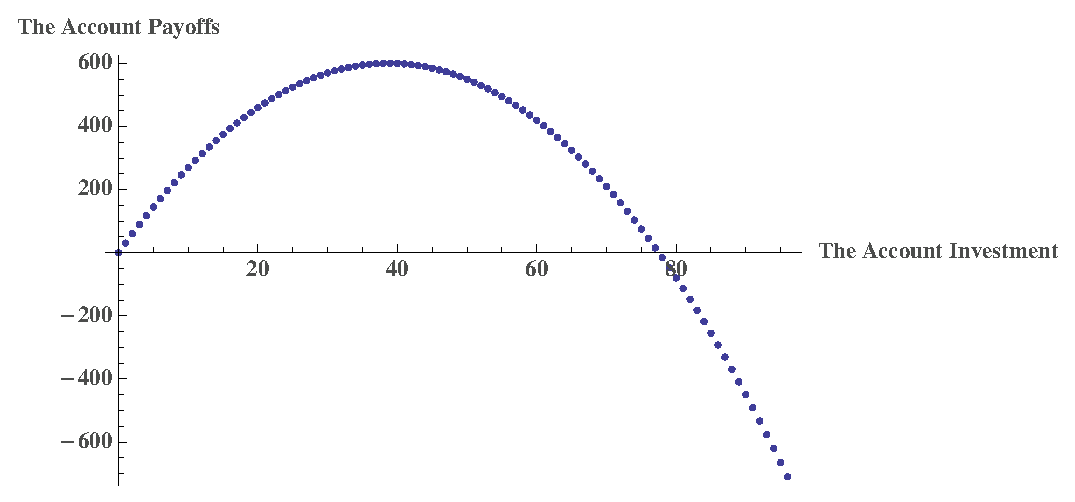
\includegraphics[width=50pc]{instructionsplot}
\caption{The Account payoff}
\end{figure}

\end{landscape}

\fi
%----------------------------------------------------------------------------------------






%----------------------------------------------------------------------------------------
\iffalse

\newpage

\begin{landscape}

{\bf \scshape Personal Record Table}


\begin{table}[H]
\centering
      \begin{tabular}{|c|p{2cm}|p{2.5cm}|p{2.5cm}|p{2cm}|p{2cm}|p{2cm}|p{2cm}|p{2.5cm}|p{2cm}|} \hline

         & {\bf Vote (Y/N)}
         & {\bf Investment}
         & {\bf Investment payoff}
         & {\bf Other \.  payoff}
         & {\bf Initial \. payoff}
         & {\bf Deduction points assigned}
         & {\bf Deduction points received}
         & {\bf Total cost of \. deduction points}
         & {\bf Final \. payoff}\\
         
         \hline\hline
         
         {\bf 1} & & & & & & & & & \\[2ex]\hline
         {\bf 2} & & & & & & & & & \\[2ex]\hline  
         {\bf 3} & & & & & & & & & \\[2ex]\hline
         {\bf 4} & & & & & & & & & \\[2ex]\hline
         {\bf 5} & & & & & & & & & \\[2ex]\hline
         {\bf 6} & & & & & & & & & \\[2ex]\hline
         {\bf 7} & & & & & & & & & \\[2ex]\hline
         {\bf 8} & & & & & & & & & \\[2ex]\hline
         {\bf 9} & & & & & & & & & \\[2ex]\hline
         {\bf 10} & & & & & & & & & \\[2ex]\hline
         
         \hline






      \end{tabular}
\end{table}

\end{landscape}

\fi
%----------------------------------------------------------------------------------------

%----------------------------------------------------------------------------------------
%	END
%----------------------------------------------------------------------------------------
\end{document}
